\section{Experiments}

We train STELLAR on ImageNet-1K~\citep{deng2009imagenet} without labels. The encoder is a vanilla ViT~\citep{dosovitskiy2020image} augmented with $8$–$24$ learnable latent queries that produce sparse tokens. A lightweight $6$-layer ViT serves as the decoder predicting either MaskGIT-VQGAN tokens~\citep{esser2021taming, chang2022maskgit}. When using a foundation prior for the backbone ViT, we ensure that the pretraining was also performed only on ImageNet-1K. We use MAE as the default prior and studied the effect of different prior modes in ablation study. When training from random prior, we use a momentum updated encoder to encode the target assignments $\tilde{q}$ in \eqref{eq-cluster} and \eqref{eq-align}, following \citeauthor{grill2020bootstrap, caron2021emerging}. 

\begin{figure*}
    \centering
    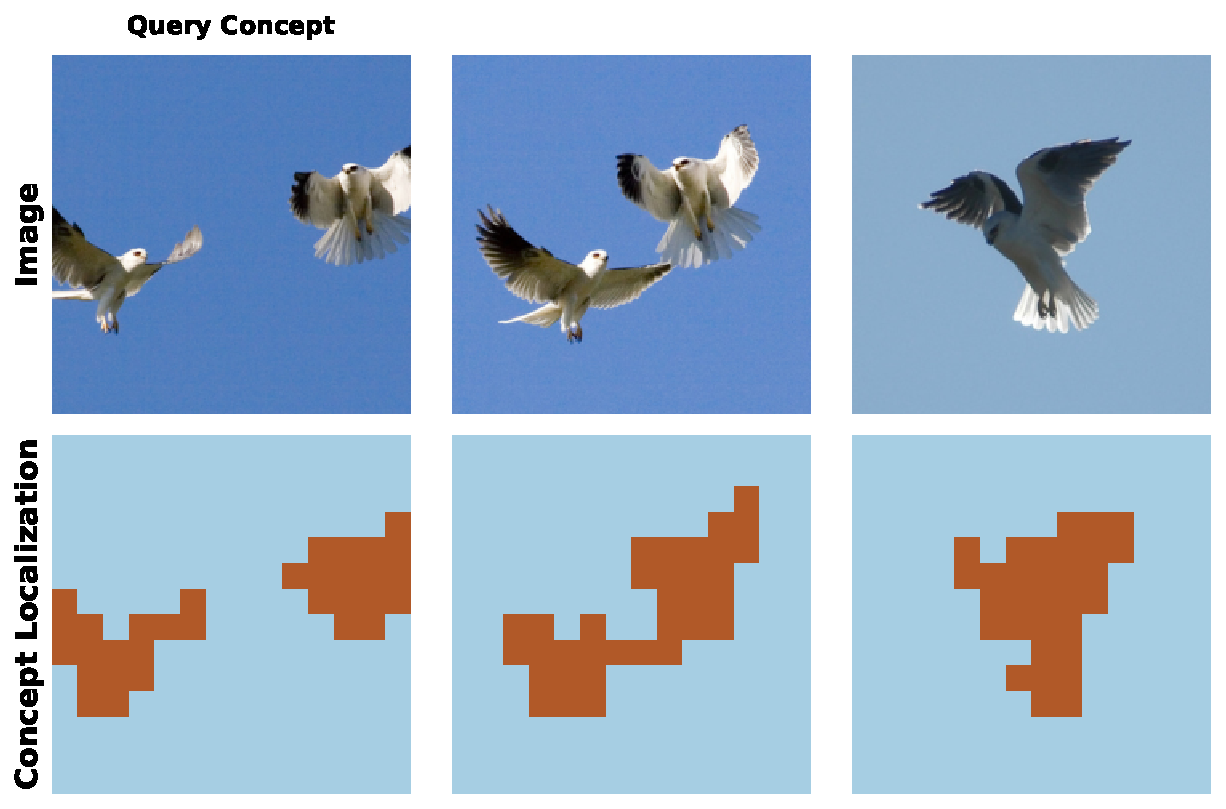
\includegraphics[width=0.49\linewidth]{figures/stellar_spatial_correspondence.pdf}
    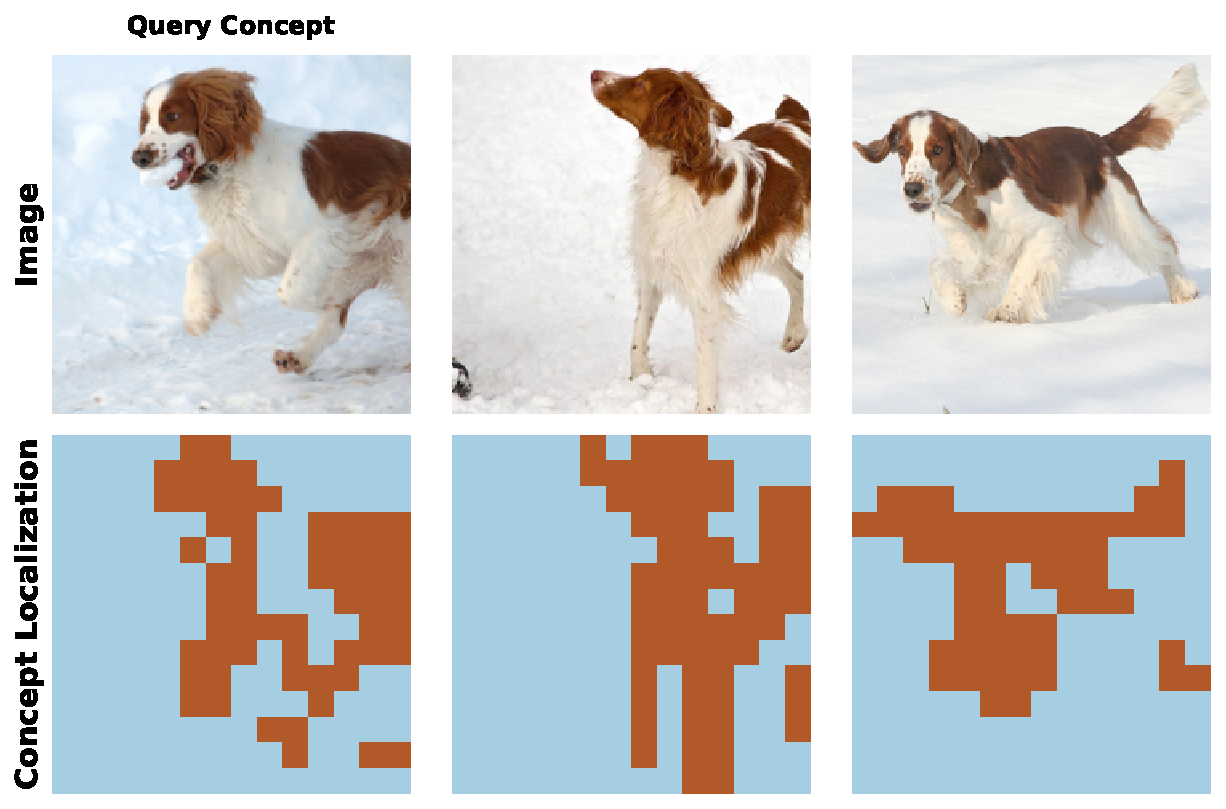
\includegraphics[width=0.49\linewidth]{figures/stellar_spatial_correspondence_1.pdf}
    \caption{Vision concepts retrieved from the training set. We show show both the image and the spatial localization of the concept.}
    \label{fig:retrieve}
\end{figure*}

\subsection{Probing the Factorized Representation}

We designed a series of experiments to analyzed the factorized representation $\mZ = \mL \mS$ from STELLAR training. 

\paragraph{Experiment 1: Equivariant Partitioning}
We built a controllable and parametrized spatial transformation group to examine the equivariant partitioning in \eqref{eq:factorized_equivariance}. Given an image, we take a crop and shift it gradually from 5 to 30 pixel, either horizontally or vertically. We calculated the relative matrix difference $\frac{\|\mS(t_\theta \circ X) - \mS( X)\|_F}{\|\mS( X)\|_F}$ and $\frac{\|\mL(t_\theta \circ X) - \mL( X)\|_F}{\|\mL( X)\|_F}$. Optimal tsansport in \eqref{eq-match} is used to match the token ordering. As shown in Fig.~\ref{fig:analysis}(a), the semantic matrix $\mS$ stays almost completely invariant, while the spatial localization matrix $\mL$ changes continuously with the spatial shift, proving the effectiveness of equivariant partitioning in the factorized representation.
\paragraph{Experiment 2: Transformation Robustness} 
Next we compare the semantic stability of STELLAR representation with baseline models under random resized cropping at scale 50-100\%. We calculate the cosine distance from the feature of the untransformed image as a measure of semantic instability. For DINO and MAE, we used mean-pooled dense features, and for sparse models STELLAR and TiTok, we used mean-pooled sparse tokens. As shown in Fig.~\ref{fig:analysis}(b), the sparse tokens of STELLAR enjoys high transformation robustness at DINO level. As expected, the reconstruction-based models MAE and TiTok show higher variance to spatial transformation. Specifically, the un-factorized sparse representation from TiTok is extremely unstable, as the model need to store both semantic and spatial information in the same sparse tokens for reconstruction.
\paragraph{Experiment 3: Effect of Low-rank Bottleneck} 
The number of sparse tokens $r$ serves as the intrinsic rank of the latent representation. We experimented scaling $r$
from 8 to 24, and evaluated reconstruction with FID~\citep{NIPS2017_8a1d6947} and semantics with linear probing on mean-pooled sparse tokens. As shown in Fig.~\ref{fig:analysis}(c), the linear probing accuracy decreases as $r$ increases, while reconstruction improves with more tokens, showing a trade-off in the intrinsic rank of the representation. As a sweet spot, $r=16$ enjoys both rich semantics and high-quality reconstruction, which we used as the default for all other experiments.

Finally, we visualize the factorized representation in Fig.~\ref{fig:retrieve}. We show the spatial localization (thresholded by $1/r$) of a sparse token in the image, and the top retrieved semantic concepts from the training dataset.


\subsection{Evaluating Holistic Representation}

Next we examine the semantic quality and reconstruction potential of representation from different models. We trained the same decoder in STELLAR on top of the frozen features from different encoders. The original decoder in STELLAR was also finetuned with the rest of the model frozen. TiTok used it's native decoder, which is a full-sized ViT compared to only 6 layers in STELLAR.

As shown in Table~\ref{fid-acc-table}, STELLAR (shown as ours) shows superior performance in supporting both semantics and reconstruction. The linear probing and k-NN accuracy of STELLAR surpass reconstruction-feasible representations from all baselines, despite trailing behind the CLS token from DINO, which is infeasible as a reconstruction latent. 


% Table \ref{fid-acc-table} and Figure \ref{fig:tokens} shows results across token counts ($8$, $16$, $24$), compared with TiTok~\citep{yu2024image} and MAE~\citep{he2022masked}. STELLAR achieves strong reconstruction even with few tokens (rFID $=3.68$ with $8$ tokens; $2.60$ with ViT-H, $16$ tokens), approaching MaskGIT-VQGAN ($2.28$) without decoder finetuning. For linear probing, STELLAR maintains robust accuracy and does not drop with more tokens as in TiTok~\citep{yu2024image}. Reconstruction improves with the number of token, but plateau after 16. We used 16 tokens in all other experiments unless specified. We also see in Figure \ref{fig:tokens} that STELLAR preserves the location of the objects. Interestingly, it also automatically removes the dark edge in the bottom example, indicating it is reconstructing from high-level semantics rather than memorizing low-level details. Overall, STELLAR balances efficient reconstruction and discriminative understanding at high quality.

\begin{table}[h]
\caption{Reconstruction and semantic metrics on IN1K of STELLAR (ours) and baseline models. For reference, we also reported semantic metrics of the global representation from DINO, and huge size STELLAR model. Best main results are shown in \textbf{bold}. Model sizes are ViT-B by default, with larger sizes indicated in parentheses. *: TiTok used its native ViT decoder of larger size.}
\label{fid-acc-table}
\begin{center}
\begin{small}
\begin{sc}
\begin{tabular}{lc|cc|cc}
\toprule
\multicolumn{2}{c}{} & \multicolumn{2}{c}{Reconstruction} & \multicolumn{2}{c}{Semantics} \\
\midrule
Model  & \# tks & FID $\downarrow$ & LPIPS $\downarrow$ & Lin. & kNN \\
\midrule
DINO & 1 & - & - & \color{gray}{76.46}& \color{gray}{74.69}\\
DINO & 196 & 3.27 & 0.2121 & 70.31 & 54.41 \\
MAE & 196 & 3.02 & \textbf{0.2071}& 66.32 & 25.82 \\
TiTok* & 32 & 2.75 & 0.3281 & 33.42 & 7.30 \\
TiTok* & 64 & 1.99 & 0.2571 & 32.87 & 7.29 \\
\midrule
ours & 16 & 3.06 & 0.2077 & \textbf{73.26}& \textbf{67.25}\\
ours & 196 & \textbf{2.85}& 0.2085 & 72.21 & 64.71 \\
ours(H)& 16 & 2.60& 0.1729& 79.10& 77.31\\
\bottomrule
\end{tabular}
\end{sc}
\end{small}
\end{center}
\vskip -0.1in
\end{table}

On reconstruction, STELLAR shows comparable FID and LPIPS loss~\cite{zhang2018unreasonable} to the dense feature map from MAE, with 90\% reduction in latent size. Although TiTok achieved lower FID with a much larger decoder, its shows highest LPIPS loss, indicating poor spatial consistency. In contrast, STELLAR exhibits superior reconstruction locality even with fewer tokens. The full-rank dense feature map $\mU$ (196 tokens) from the ViT in STELLAR shows even lower reconstruction FID, while drops in semantic quality. Finally, when scaling to huge-sized ViT, STELLAR achieves top reconstruction and semantic quality, even without decoder finetuning.

\subsection{Benchmarking Image Understanding}

Lastly, we benchmark STELLAR in classical image understanding tasks with linear probing on frozen features, comparing against other ImageNet-pretrained SSL models. We report results for classification on ImageNet-1K (IN1K), Oxford-IIIT Pet (Pets)~\citep{parkhi2012cats}, Food-101 (Food)~\citep{bossard14}, and GlaS~\citep{sirinukunwattana2016gland} for cancer grade classification in histopathology. Segmentation benchmarks include ADE20K~\citep{zhou2017scene}, Cityscapes~\citep{cordts2016cityscapes}, and Pascal VOC~\citep{everingham2010pascal}.  For broader context, we also include AIM~\citep{el2024scalable} and DINOv2~\citep{oquab2023dinov2}, which leverage substantially larger training corpora (100–1000$\times$ more images).





\begin{table*}[t]
\caption{\textbf{Evaluation of Fine-grained and Global Image Understanding.} We evaluate semantic segmentation (mIoU \%) and classification accuracy (\%) via linear probing on frozen features. We used the dense feature map from the backbone for all segmentation tasks and all models. \textbf{Bold}: best with ImageNet training. \underline{Underline}: best in architectural class (e.g., ViT-B).}
\label{tab:merged_results}
\begin{center}
\begin{small}
\begin{sc}
% \setlength{\tabcolsep}{3.5pt}
\begin{tabular}{l l c c | c c c | c c c c}
\toprule
& & \multicolumn{2}{c|}{\bf SSL Type} & \multicolumn{3}{c|}{\bf Segmentation (mIoU)} & \multicolumn{4}{c}{\bf Classification (Acc)} \\
\bf Model & \bf Arch. & \bf Target & \bf Method & \bf ADE20K & \bf CitySc & \bf VOC & \bf IN1K & \bf Pets & \bf Food & \bf GlaS \\
\midrule
\multicolumn{11}{l}{\it Semantic-Centric (Joint Embedding / Invariance)} \\
BYOL & RN-50 & Global & Distill & 18.43 & \underline{18.66} & 63.89 & \underline{70.39} & \underline{82.77} & \underline{64.57} & \underline{95.00} \\
MoCo v3 & ViT-B & Global & Contr. & 29.45 & 25.13 & 74.08 & 74.31 & 91.14 & 77.47 & \textbf{97.50} \\
DINO & ViT-B & Global & Distill & 26.87 & 26.82 & 79.29 & \underline{76.46} & \textbf{93.84} & \underline{79.28} & 95.00 \\
MSN & ViT-B & Global & Masking & 26.66 & 25.39 & 68.59 & 73.65 & 75.91 & 68.93 & 92.50 \\
DenseCL & RN-50 & Dense & Contr. & \underline{23.08} & 18.63 & \underline{70.95} & 61.10 & 72.99 & 59.16 & 85.00 \\
Data2Vec & ViT-B & Dense & Lat-MIM & 22.03 & 23.49 & 61.33 & 54.90 & 26.47 & 34.40 & 73.75 \\
SiameseIM & ViT-B & Dense & Lat-MIM & 29.24 & 26.52 & 81.38 & 74.97 & 91.61 & 71.01 & 91.25 \\
I-JEPA & ViT-H & Dense & Lat-MIM & 21.57 & 18.59 & 74.13 & 71.72 & 84.68 & 70.34 & 87.50 \\
iBOT & ViT-B & Gl+De & Dist+MIM & \underline{31.78} & 25.69 & 77.06 & 76.40 & 92.40 & 78.08 & 96.25 \\
iBOT & ViT-L & Gl+De & Dist+MIM & 33.26 & 26.37 & 77.57 & \underline{78.53} & 92.12 & \textbf{81.07} & 96.25\\
\midrule
\multicolumn{11}{l}{\it Image-Centric (Reconstruction)} \\
BEIT & ViT-B & Dense & Tok MIM & 11.58 & 18.90 & 27.44 & 32.94 & 36.20 & 54.49 & 90.00 \\
BEIT & ViT-L & Dense & Tok MIM & 12.64 & 20.37 & 25.48 & 36.77 & 36.71 & 56.03 & 90.00 \\
SimMIM & Swin-B & Dense & Pix MIM & 12.46 & 17.23 & 35.14 & 24.77 & 27.39 & 40.94 & 77.50 \\
MAE & ViT-B & Dense & Pix MIM & 30.91 & \underline{29.44} & 76.43 & 66.32 & 81.58 & 70.40 & 93.75 \\
MAE & ViT-L & Dense & Pix MIM & \underline{34.36} & \underline{32.53} & 77.79 & 73.09 & 84.30 & 76.22 & 95.00 \\
MAE & ViT-H & Dense & Pix MIM & 36.16 & \bf{35.21} & 78.07 & 75.22 & 84.96 & \underline{78.36} & \underline{95.00} \\
SemMAE & ViT-B & Dense & Pix MIM & 3.52 & 25.48 & 48.33 & 43.84 & 56.99 & 58.90 & 92.50 \\
TiTok-64 & ViT-B & Sparse & Sprs Rec & -- & -- & -- & 32.87 & 42.06 & 43.68 & \textbf{97.50} \\
TiTok-32 & ViT-L & Sparse & Sprs Rec & -- & -- & -- & 33.42 & 27.83 & 38.83 & 78.75 \\
\midrule
\multicolumn{11}{l}{\it Our Method (Sparse Factorized Modeling)} \\
\bf STELLAR & ViT-B & Sparse & Inv+Rec & 31.33 & 27.74 & \underline{81.83} & 73.26 & 89.70 & 74.09 & 95.00 \\
\bf STELLAR & ViT-L & Sparse & Inv+Rec & 34.02 & 31.32 & \textbf{85.90} & 76.94 & \underline{92.53} & 74.78 & \textbf{97.50} \\
\bf STELLAR & ViT-H & Sparse & Inv+Rec & \textbf{36.66} & 33.30 & \underline{85.66} & \textbf{79.10} & \underline{92.53} & 77.43 & 92.50 \\
\midrule
\multicolumn{11}{l}{\it Larger Scale Pretraining Beyond ImageNet (Reference Only)} \\
AIM & 600 M & Dense & Image AR & 29.00 & 27.04 & 64.55 & 63.78 & 64.68 & 75.19 & 98.75 \\
AIM & 1 B & Dense & Image AR & 29.59 & 27.05 & 63.90 & 66.86 & 64.21 & 77.96 & 96.25 \\
DINOv2 & ViT-B* & Gl+De & Dist+MIM & 40.10 & 34.66 & 89.52 & 82.82 & 95.59 & 91.08 & 98.75 \\
DINOv2 & ViT-L* & Gl+De & Dist+MIM & 40.45 & 32.07 & 89.19 & 84.23 & 96.08 & 92.94 & 98.75 \\
\bottomrule
\end{tabular}
\end{sc}
\end{small}
\end{center}
\vskip -0.1in
\end{table*}

As shown in Table \ref{tab:merged_results}, the feature map from STELLAR achieves superior performance on ADE20K and Pascal VOC, showing strong fine-grained understanding despite not applying SSL objectives directly to the dense feature map $\mU$. Sparse token modeling implicitly organizes the feature map into semantic regions: to reconstruct the image, each token must encode information covering all spatial parts of the scene, resulting in region-aware representations. While MAE leads in CityScapes, STELLAR follows closed with performance comparable to MAE and DINOv2. 



On global image understanding tasks, STELLAR achieves the highest accuracy on IN1K at large model scale, but smaller variants underperform methods such as DINO, which explicitly optimizes for global representations. In general, STELLAR outperforms image reconstruction models and most JE methods, but trails behind top JE models in global semantics. As we do not model the image as a single concept, averaging token features can dilute discriminative information, which is particularly detrimental on object-centric datasets like Pets and Food. Interestingly, on histopathology images involving complex tissue microenvironments, STELLAR achieves the best performance. These results indicate that STELLAR excels at modeling complex, multi-object scenes, while global classification on simple object-centric datasets remains more challenging.



% \begin{table*}[t]
% \caption{\small Ablation on IN1K linear probing accuracy (\%) and ADE20K linear probing mIOU (\%).}
% \label{ablation-table}
% \begin{center}
% \begin{small}
% \begin{sc}
% \begin{tabular}{ccccc|ccc}
% \multicolumn{1}{c}{Recon.}  &\multicolumn{1}{c}{Cluster} &  Set align & CLS align & KoLeo & Recon FID $\downarrow$  & IN1K lin. & ADE20K lin. \\
% \hline 
% \multicolumn{7}{l}{\it Default} \\
%    \checkmark    & \checkmark  & \checkmark & \checkmark & \checkmark & 3.14 & 73.26 & 31.33\\
% \hline 
% \multicolumn{7}{l}{\it Ablation model versions} \\
%  \ding{55}   & \checkmark  & \checkmark & \checkmark & \checkmark & - & 72.44 (-0.82) & 29.94 (-1.39) \\
%  \checkmark    &  \ding{55}   &  \ding{55}  &  \ding{55}  & \checkmark & 3.21 (+0.07) & 52.07 (-21.19) & 20.46 (-10.87) \\
%  \checkmark    & \checkmark  & \ding{55}  & \ding{55}  & \checkmark & 8.95 (+5.81) & 2.73 (-70.53) & 1.93 (-29.39) \\
%  \checkmark    &  \ding{55} & \checkmark  & \checkmark  & \checkmark & 3.62 (+0.48) & 42.14 (-31.12) & 18.90 (-12.43) \\
%   \checkmark    & \checkmark  & \checkmark & \ding{55}  & \checkmark & 3.26 (+0.12) & 70.79 (-2.47) & 30.20 (-1.12) \\
%   \checkmark    & \checkmark  & \checkmark & \checkmark & \ding{55}  & 3.25 (+0.11) & 72.05 (-1.21) & 30.10 (-1.23) \\
% \end{tabular}
% \end{sc}
% \end{small}
% \end{center}
% \vskip -0.1in
% \end{table*}

\begin{table*}[t]
\caption{\textbf{Ablation.} We isolate the impact of each objective on semantic abstraction (IN1K) and spatial grounding (ADE20K), and reconstruction (FID). \textit{Default} denotes the full STELLAR framework. All results are based on ViT-B.}
\label{ablation-table}
\begin{center}
\begin{small}
\begin{sc}
% \setlength{\tabcolsep}{3.8pt}
\begin{tabular}{l ccccc | ccc}
\toprule
& \bf Recon. & \bf Cluster & \bf Set Align& \bf CLS Align& \bf KoLeo & \bf rFID $\downarrow$ & \bf IN1K $\uparrow$ & \bf ADE $\uparrow$ \\
\midrule
Default & \checkmark & \checkmark & \checkmark & \checkmark & \checkmark & \bf 3.14 & \bf 73.26 & \bf 31.33 \\
\midrule
\multicolumn{9}{l}{\it Impact of Individual Components} \\
(a) & \ding{55} & \checkmark & \checkmark & \checkmark & \checkmark & --- & 72.44 \color{gray}{(-0.82)} & 29.94 \color{gray}{(-1.39)} \\
(b) & \checkmark & \ding{55} & \ding{55} & \ding{55} & \checkmark & 3.21 \color{gray}{(+0.07)} & 52.07 \color{red}{(-21.19)} & 20.46 \color{red}{(-10.87)} \\
(c) & \checkmark & \checkmark & \ding{55} & \ding{55} & \checkmark & 8.95 \color{red}{(+5.81)} & 2.73 \color{red}{(-70.53)} & 1.93 \color{red}{(-29.39)} \\
(d) & \checkmark & \ding{55} & \checkmark & \checkmark & \checkmark & 3.62 \color{gray}{(+0.48)} & 42.14 \color{red}{(-31.12)} & 18.90 \color{red}{(-12.43)} \\
(e) & \checkmark & \checkmark & \checkmark & \ding{55} & \checkmark & 3.26 \color{gray}{(+0.12)} & 70.79 \color{gray}{(-2.47)} & 30.20 \color{gray}{(-1.12)} \\
(f) & \checkmark & \checkmark & \checkmark & \checkmark & \ding{55} & 3.25 \color{gray}{(+0.11)} & 72.05 \color{gray}{(-1.21)} & 30.10 \color{gray}{(-1.23)} \\
\bottomrule
\end{tabular}
\end{sc}
\end{small}
\end{center}
\vskip -0.1in
\end{table*}

\subsection{Ablation Analysis}
\textbf{Low-rank approximated reconstruction.}
As shown in Table~\ref{ablation-table}, removing the low-rank reconstruction objective (A) reduces both global and fine-grained understanding. Since the remaining objectives resemble typical SSL methods, the model still retains reasonable global performance, but fine-grained understanding suffers more. This indicates that low-rank reconstruction encourages sparse tokens to serve as holistic representations covering the entire image.

\textbf{Concept clustering.}
Eliminating online clustering and set alignment (B) leads to a sharp drop in understanding, highlighting the necessity of structuring sparse tokens into view-invariant concepts. Even when the alignment loss is present (D), missing the clustering loss still lead to feature collapse. 

\textbf{Set alignment.}
The training collapsed when training with only reconstruction and clustering (C), underscoring the critical role of set concepts alignment. Additional alignment on the CLS token (E) primarily benefits global classification but has limited effect on spatial grounding. Finally, KoLeo regularization (F) consistently improves all tasks at similar level. Interestingly, the absent of either concept clustering or set alignment led to a sharp drop in performance.

\textbf{Foundational Prior} We ablated STELLAR trained from different pretrained foundational prior in Table \ref{init-table}. We observes that STELLAR significantly boost the semantic quality from MAE, and the spatial grounding from DINO prior. The semantics performance falls to similar level despite different foundational priors. When training from random prior, STELLAR is able to reach semantics at MAE level and spatial understanding similar to that from DINO prior. The reconstruction quality stays consistent in all cases.



% \begin{table*}[ht]
% \caption{Ablation on model initialization and training strategy}
% \label{init-table}
% \begin{center}
% \begin{small}
% \begin{sc}
% \begin{tabular}{c|cc|ccccccccc}
% \multicolumn{1}{c}{} & \color{gray}{MAE} & \color{gray}{DINO}  & MAE init. & DINO init. & EMA only & EMA+75ep. \\
% \hline 
% Recon. FID ($\downarrow$) & - & - & 3.14 & 3.31 & 3.69 & 3.21 \\
% Class. Acc. & \color{gray}{66.32} & \color{gray}{76.46} &  73.26 & 73.31 & 58.83  & 65.28 \\
% Seg. mIOU & \color{gray}{30.91} & \color{gray}{26.87} &  31.33 & 28.17 & 26.79 & 28.10 \\
% \end{tabular}
% \end{sc}
% \end{small}
% \end{center}
% \end{table*}





\begin{table}[ht]
\caption{Evaluating STELLAR trained from different foundational priors. \textit{Base} represents the performance of the original backbone.}
\label{init-table}
\begin{center}
\begin{small}
\begin{sc}
\setlength{\tabcolsep}{4pt}
\begin{tabular}{l | c | cc | cc}
\toprule
&  \bf Recon & \multicolumn{2}{c|}{\bf Semantic (IN1K)} & \multicolumn{2}{c}{\bf Spatial (ADE20K)} \\
\bf Prior &  \bf FID $\downarrow$ & Base & \bf +STELLAR & Base & \bf +STELLAR \\
\midrule
MAE &  \bf 3.14 & 66.32 & \bf 73.26 \color{blue}{(+6.9)} & 30.91 & \bf 31.33 \color{blue}{(+0.4)} \\
DINO &  3.31 & 76.46 & 73.31 \color{red}{(-3.2)} & 26.87 & \bf 28.17 \color{blue}{(+1.3)} \\
\midrule
rand & 3.21 & -- & 65.28 & -- & 28.10 \\
\bottomrule
\end{tabular}
\end{sc}
\end{small}
\end{center}
\end{table}